% concatenated from bench-mfg-arxiv.tex, tikz-figures/overview.tex, utils/algo_tables-arxiv.tex
\documentclass[10pt,twocolumn,letterpaper]{article}

\usepackage[margin=0.75in]{geometry}
\usepackage{times} %
\usepackage{microtype}
\usepackage{graphicx}
\usepackage{subcaption}
\usepackage{booktabs}
\usepackage{hyperref}
\usepackage[table]{xcolor}

\usepackage{amsmath, amssymb, mathtools, amsthm}
\newtheorem{theorem}{Theorem}[section]
\newtheorem{proposition}[theorem]{Proposition}
\newtheorem{lemma}[theorem]{Lemma}
\newtheorem{corollary}[theorem]{Corollary}
\theoremstyle{definition}
\newtheorem{definition}[theorem]{Definition}
\usepackage{natbib}
\theoremstyle{remark}
\newtheorem{remark}[theorem]{Remark}
\newtheorem{example}{Example}
\usepackage{algorithm}
\usepackage{algorithmic}
\renewcommand{\algorithmicrequire}{\textbf{Input:}}
\renewcommand{\algorithmicensure}{\textbf{Output:}}

\usepackage[framemethod=tikz]{mdframed}
\usepackage{tikz}
\usetikzlibrary{positioning, calc, backgrounds, shapes.geometric, decorations.pathmorphing, shapes.callouts}
\usepackage[most]{tcolorbox}
\definecolor{darkgreen}{rgb}{0.0, 0.5, 0.0}%
\definecolor{pastelblue}{rgb}{0.30, 0.60, 0.80}
\definecolor{salmon}{rgb}{0.98, 0.50, 0.45}
\newcommand{\bsa}{{\boldsymbol{a}}}
\newcommand{\states}{\mathcal{X}}
\newcommand{\actions}{\mathcal{A}}
\newcommand{\R}{\mathbb{R}}
\newcommand{\EE}{\mathbb{E}}
\DeclareMathOperator*{\argmax}{arg\,max}
\DeclareMathOperator*{\argmin}{arg\,min}
\usepackage{hyperref}

\newcommand{\Puni}{ \cP_{\text{\tiny Unif}}}
\newcommand{\ion}{\frac{i}{n}}
\newcommand{\jon}{\frac{j}{n}}
\newcommand{\con}{\frac{C}{n}}
\newcommand{\Ion}{\frac{1}{n}}
\newcommand{\kon}{\frac{k}{n}}
\newcommand{\tX}{\widetilde{X}}
\newcommand{\talpha}{\widetilde{\alpha}}
\newcommand{\sumi}{\sum_{i=1}^n}
\newcommand{\sumj}{\sum_{j=1}^n}


\newcommand{\Q}{\mathbb{Q}}
\newcommand{\N}{\mathbb{N}}

\newcommand{\ocT}{{\overline{\cT}}}
\newcommand{\BR}{\mathbf{BR}}


\newcommand{\noises}{\mathcal{C}}
\newcommand{\exploitability}{\mathcal{E}}
\newcommand{\unif}{\mathrm{Unif}}
\newcommand{\cP}{\mathcal{P}}
\newcommand{\cR}{\mathcal{R}}
\setlength{\parindent}{0pt}      %
\setlength{\parskip}{1.2ex plus 0.5ex minus 0.2ex} %
\hypersetup{
    colorlinks=true,      %
    allcolors=blue!60!black,       %
}
\begin{document}

\twocolumn[
  \begin{center}
    {\LARGE \textbf{Bench-MFG: A Benchmark Suite for Learning\\ in Stationary Mean Field Games} \par}
    \vspace{1.5em}
    {\large Lorenzo Magnino$^1$, Jiacheng Shen$^{2,3}$, Matthieu Geist$^4$, Olivier Pietquin$^4$, Mathieu Lauri\`ere$^{5}$ \par}
    \vspace{1em}
    {\small $^1$University of Cambridge \quad $^2$NYU Shanghai \quad $^3$NYU Center for Data Science \quad $^4$Earth Species Project \par}
    {\small $^5$NYU Shanghai Center for Data Science; NYU-ECNU Institute of Mathematical Sciences at NYU Shanghai \par}
    \vspace{1.5em}
  \end{center}
]

\begin{abstract}
The intersection of Mean Field Games (MFGs) and Reinforcement Learning (RL) has fostered a growing family of algorithms designed to solve large-scale multi-agent systems. However, the field currently lacks a standardized evaluation protocol, forcing researchers to rely on bespoke, isolated, and often simplistic environments. This fragmentation makes it difficult to assess the robustness, generalization, and failure modes of emerging methods. To address this gap, we propose a comprehensive benchmark suite for MFGs (Bench-MFG), focusing on the discrete-time, discrete-space, stationary setting for the sake of clarity. We introduce a taxonomy of problem classes, ranging from no-interaction and monotone games to potential and dynamics-coupled games, and provide prototypical environments for each. Furthermore, we propose MF-Garnets, a method for generating random MFG instances to facilitate rigorous statistical testing. We benchmark a variety of learning algorithms across these environments, including a novel black-box approach (MF-PSO) for exploitability minimization. Based on our extensive empirical results, we propose guidelines to standardize future experimental comparisons. Code available at \href{https://github.com/lorenzomagnino/Bench-MFG}{https://github.com/lorenzomagnino/Bench-MFG}.
\end{abstract}
\vspace{2em}
\section{Introduction}
\begin{figure}[t]
    \centering
    \resizebox{0.5\textwidth}{!}{%
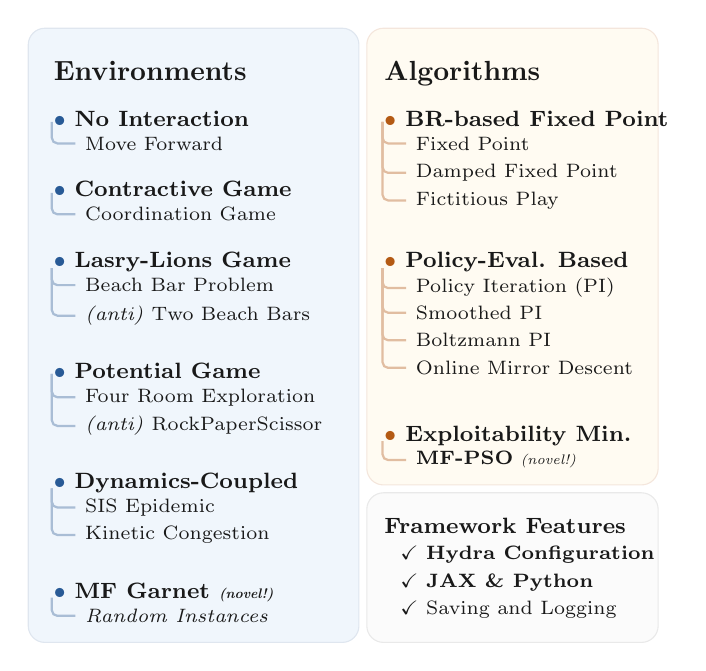
\begin{tikzpicture}[font=\sffamily, x=1cm, y=1cm]

    \definecolor{envBlue}{RGB}{40, 90, 150}      %
    \definecolor{envBg}{RGB}{240, 246, 252}     %
    \definecolor{algoOrange}{RGB}{180, 90, 20}   %
    \definecolor{algoBg}{RGB}{255, 251, 242}    %
    \definecolor{textDark}{RGB}{25, 25, 25}     %
    \definecolor{borderGray}{RGB}{200, 200, 200}

    \tikzset{
        header/.style={font=\bfseries\small, text=textDark, anchor=north west},
        parent/.style={font=\bfseries\footnotesize, text=textDark, anchor=north west, inner ysep=4pt},
        child/.style={font=\scriptsize, text=textDark, anchor=north west, inner ysep=2pt},
        connector/.style={thick, rounded corners=2pt}
    }

    \def\xParentEnv{0}
    \def\xChildEnv{0.4}
    
    \node[header, font=\bfseries\normalsize] (EnvTitle) at (\xParentEnv, 0) {Environments};

    \node[parent] (NI) at (\xParentEnv, -0.6) {\textcolor{envBlue}{$\bullet$} No Interaction};
    \node[child] (NI_1) at (\xChildEnv, -1.0) {Move Forward};
    \draw[connector, draw=envBlue!40] (NI.south west) ++(0.1,0.2) |- (NI_1.west);

    \node[parent] (Cont) at (\xParentEnv, -1.5) {\textcolor{envBlue}{$\bullet$} Contractive Game};
    \node[child] (Cont_1) at (\xChildEnv, -1.9) {Coordination Game};
    \draw[connector, draw=envBlue!40] (Cont.south west) ++(0.1,0.2) |- (Cont_1.west);

    \node[parent] (LL) at (\xParentEnv, -2.4) {\textcolor{envBlue}{$\bullet$} Lasry-Lions Game};
    \node[child] (LL_1) at (\xChildEnv, -2.8) {Beach Bar Problem};
    \node[child] (LL_2) at (\xChildEnv, -3.15) {\textit{(anti)} Two Beach Bars};
    \draw[connector, draw=envBlue!40] (LL.south west) ++(0.1,0.2) |- (LL_1.west);
    \draw[connector, draw=envBlue!40] (LL.south west) ++(0.1,0.2) |- (LL_2.west);

    \node[parent] (Pot) at (\xParentEnv, -3.8) {\textcolor{envBlue}{$\bullet$} Potential Game};
    \node[child] (Pot_1) at (\xChildEnv, -4.2) {Four Room Exploration};
    \node[child] (Pot_2) at (\xChildEnv, -4.55) {\textit{(anti)} RockPaperScissor};
    \draw[connector, draw=envBlue!40] (Pot.south west) ++(0.1,0.2) |- (Pot_1.west);
    \draw[connector, draw=envBlue!40] (Pot.south west) ++(0.1,0.2) |- (Pot_2.west);

    \node[parent] (DC) at (\xParentEnv, -5.2) {\textcolor{envBlue}{$\bullet$} Dynamics-Coupled};
    \node[child] (DC_1) at (\xChildEnv, -5.6) {SIS Epidemic};
    \node[child] (DC_2) at (\xChildEnv, -5.95) {Kinetic Congestion};
    \draw[connector, draw=envBlue!40] (DC.south west) ++(0.1,0.2) |- (DC_1.west);
    \draw[connector, draw=envBlue!40] (DC.south west) ++(0.1,0.2) |- (DC_2.west);

    \node[parent] (Gar) at (\xParentEnv, -6.6) {\textcolor{envBlue}{$\bullet$} MF Garnet \textit{\tiny (novel!)}};
    \node[child] (Gar_1) at (\xChildEnv, -7.0) {\textit{Random Instances}};
    \draw[connector, draw=envBlue!40] (Gar.south west) ++(0.1,0.2) |- (Gar_1.west);

    \def\xParentAlgo{4.2}
    \def\xChildAlgo{4.6}

    \node[header, font=\bfseries\normalsize] (AlgoTitle) at (\xParentAlgo, 0) {Algorithms};

    \node[parent] (BR) at (\xParentAlgo, -0.6) {\textcolor{algoOrange}{$\bullet$} BR-based Fixed Point};
    \node[child] (BR_1) at (\xChildAlgo, -1.0) {Fixed Point};
    \node[child] (BR_2) at (\xChildAlgo, -1.35) {Damped Fixed Point};
    \node[child] (BR_3) at (\xChildAlgo, -1.7) {Fictitious Play};
    \draw[connector, draw=algoOrange!40] (BR.south west) ++(0.1,0.2) |- (BR_1.west);
    \draw[connector, draw=algoOrange!40] (BR.south west) ++(0.1,0.2) |- (BR_2.west);
    \draw[connector, draw=algoOrange!40] (BR.south west) ++(0.1,0.2) |- (BR_3.west);

    \node[parent] (PE) at (\xParentAlgo, -2.4) {\textcolor{algoOrange}{$\bullet$} Policy-Eval. Based};
    \node[child] (PE_1) at (\xChildAlgo, -2.8) {Policy Iteration (PI)};
    \node[child] (PE_2) at (\xChildAlgo, -3.15) {Smoothed PI};
    \node[child] (PE_3) at (\xChildAlgo, -3.5) {Boltzmann PI};
    \node[child] (PE_4) at (\xChildAlgo, -3.85) {Online Mirror Descent};
    \draw[connector, draw=algoOrange!40] (PE.south west) ++(0.1,0.2) |- (PE_1.west);
    \draw[connector, draw=algoOrange!40] (PE.south west) ++(0.1,0.2) |- (PE_2.west);
    \draw[connector, draw=algoOrange!40] (PE.south west) ++(0.1,0.2) |- (PE_3.west);
    \draw[connector, draw=algoOrange!40] (PE.south west) ++(0.1,0.2) |- (PE_4.west);

    \node[parent] (Exp) at (\xParentAlgo, -4.6) {\textcolor{algoOrange}{$\bullet$} Exploitability Min.};
    \node[child] (Exp_1) at (\xChildAlgo, -5.0) {\textbf{MF-PSO} \textit{\tiny (novel!)}};
    \draw[connector, draw=algoOrange!40] (Exp.south west) ++(0.1,0.2) |- (Exp_1.west);

    \def\yNotesStart{-5.8}
    \node[header, font=\bfseries\footnotesize] (NotesTitle) at (\xParentAlgo, \yNotesStart) {Framework Features};
    \node[child, font=\scriptsize] (Note1) at (\xParentAlgo+0.2, \yNotesStart-0.4) {$\checkmark$ \textbf{Hydra Configuration}};
    \node[child, font=\scriptsize] (Note2) at (\xParentAlgo+0.2, \yNotesStart-0.75) {$\checkmark$ \textbf{JAX \& Python}};
    \node[child, font=\scriptsize] (Note3) at (\xParentAlgo+0.2, \yNotesStart-1.1) {$\checkmark$ Saving and Logging};

    \begin{scope}[on background layer]
        \draw[fill=envBg, draw=envBlue!15, rounded corners=6pt] (-0.2, 0.3) rectangle (4.0, -7.5);
        \draw[fill=algoBg, draw=algoOrange!15, rounded corners=6pt] (4.1, 0.3) rectangle (7.8, -5.5);
        \draw[fill=gray!3, draw=borderGray!40, rounded corners=6pt] (4.1, -5.6) rectangle (7.8, -7.5);
    \end{scope}

\end{tikzpicture}
    }
    \caption{\small \textbf{Bench-MFG} Overview}
    \vspace{-0.5cm}
\end{figure}
The scalability of Multi-Agent Reinforcement Learning (MARL) remains a fundamental obstacle in the pursuit of intelligent decentralized systems. While Deep Reinforcement Learning (DRL) has demonstrated superhuman performance in zero-sum games such as Go and Chess~\citep{silver2016mastering,silver2017masteringchess}, and complex team-based environments like StarCraft~\citep{samvelyan2019starcraft}, these successes rarely translate effortlessly to systems with massive populations. As the number of agents increases, the joint state-action space expands exponentially, rendering standard MARL approaches computationally infeasible~\citep{busoniu2008comprehensive,yang2020overview,zhang2021multi}.

The Mean Field Game (MFG) framework, pioneered by~\citet{MR2295621} and~\citet{huang2006largeMKV}, circumvents this curse of dimensionality by invoking a continuum approximation. Rather than modeling pairwise interactions, MFGs focus on a representative agent interacting with the statistical distribution of the population. This formulation has proven efficient in domains requiring the modeling of large crowds, such as finance~\citep{cardaliaguet2018mean,carmona2017mean}, economics~\citep{MR2647032,achdou2022income}, and epidemiology~\citep{laguzet2015individual,olmez2022modeling,aurell2022optimal}. In the stationary setting, the problem reduces to finding a fixed point: a Nash Equilibrium where the agent's optimal policy induces a stationary distribution that, in turn, justifies the policy.

Historically, MFGs were solved using numerical methods for partial differential equations (PDEs)~\citep{achdou2020mean}. However, these grid-based methods struggle in high-dimensional state spaces. Consequently, the research community has pivoted toward learning-based approaches that leverage RL to solve MFGs without knowledge of the underlying model dynamics~\citep{guo2019learningMFG,subramanian2019reinforcementMFG,cui2021approximately}. Recent surveys~\citep{lauriere2022learning} highlight a surge in algorithms adapting well-known methods such as Fictitious Play (FP)~\citep{perrin2021meanflock,lauriere2022scalable,magnino2025solving}, Actor-Critic architectures~\citep{fu2019actorcriticMFG,angiuli2020unifiedRLMFGMFC} and Online Mirror Descent~\citep{hadikhanloo2018learningphd,perolat2021scalingMFGOMD} to this setting.

\textbf{Challenges.} Despite this methodological progress, empirical evaluation in the MFG literature remains fragmented. Unlike general RL, which benefits from standardized benchmarks like the Arcade Learning Environment~\citep{bellemare2013arcade}, MuJoCo~\citep{todorov2012mujoco}, BenchMARL ~\citep{bettini2024benchmarl} or ~\cite{gorsane2022towards}, \textbf{MFG algorithms are typically evaluated on ad-hoc, isolated examples}. These environments, often limited to Linear-Quadratic (LQ) models or simple grid worlds, fail to capture the rich diversity of interaction types found in real-world applications. For instance, an algorithm that succeeds in a monotonic setting (where congestion is penalized) may fail catastrophically in games with cyclical dynamics or complex coupling between the population distribution and state transitions.

In this work, we address the lack of a unified evaluation framework by proposing a benchmark suite specifically designed for stationary MFGs. Our contributions are: \looseness=-1
\begin{mdframed}[
    linecolor=blue!20,      %
    linewidth=0pt,        %
    roundcorner=5pt,        %
    backgroundcolor=blue!5, 
    innertopmargin=7pt, 
    innerbottommargin=5pt
]
\begin{enumerate}
    \item \textbf{Taxonomy and Prototypical Examples:} We categorize MFGs into classes based on their mathematical structure, No-Interaction, Lasry-Lions Monotone, Potential, and Dynamics-Coupled games. For each, we provide open-source, prototypical environments that isolate specific algorithmic challenges (our JAX implemenation gives 2000x of speedup compared to classical open-source methods).
    \item \textbf{Procedural Generation (MF-Garnets):} We introduce MF-Garnets. This generator constructs random MFG instances with controllable density and interaction types (additive vs. multiplicative), enabling statistical stress-testing of solvers beyond fixed examples.
    \item \textbf{Systematic Evaluation:} We benchmark a wide range of algorithms, including Fixed Point Iteration, Policy Iteration, and a novel black-box exploitability minimizer (MF-PSO), across our suite.
    \item \textbf{Guidelines:} We synthesize our findings into a set of best practices to foster reproducibility and rigor in future MFG research.
\end{enumerate}
\end{mdframed}


\section{Model}


\noindent\textbf{Notation.} If  $\mathcal L$ is a finite set, $\Delta_{\mathcal L}$ denotes the set of probability distributions on $\mathcal L$; $\unif(\mathcal{L})$ denotes the uniform distribution over $\mathcal{L}$. $P^\top$ denotes the transpose of a matrix $P$. $\mathbb N := \{0,1,2,\dots\}$.

\noindent\textbf{MFG model.} We focus on stationary models with discounted cumulative reward. A {\bf mean field game (MFG) model} is defined by a tuple $(\states, \actions, p, r, \gamma)$ where:
$\states, \actions$ are the finite state space and action space,
$p: \states \times \actions \times \Delta_{\states} \to \Delta_{\states}$ is the one-step transition probability kernel,
$r: \states \times \actions \times \Delta_{\states} \to \mathbb R$ is the one-step reward function,
$\gamma \in [0,1)$ is the discount factor. 
Instead of $p$, it is often convenient to write:
\(
    x_{n+1} = F(x_n, a_n, \mu_n, \epsilon_n), \quad \epsilon_n \sim \xi \in \Delta_{\noises} \text{ i.i.d.},
\)
where $F: \states \times \actions \times \Delta_{\states} \times \noises \to \states$ is a {\bf transition function}, $\xi$ is the noise distribution and $\noises$ is the noise space, 
so that $p(x'|x,a,\mu) = \xi(\{ e \in \noises : F(x,a,\mu,e) = x' \})$.

\noindent\textbf{Policies.} Let $\Pi = (\Delta_\actions)^{\states} = \Delta_\actions^{\states}$ denote the set of stationary policies. A policy $\pi \in \Pi$ maps a state $x \in \states$ to a distribution $\pi(\cdot|x) \in \Delta_\actions$.

\noindent\textbf{Objective function.} Assume the population distribution is stationary and given by $\mu \in \Delta_{\states}$. The {\bf total discounted reward} for a player using policy $\pi \in \Pi$ facing $\mu$ is:
\begin{equation}\label{eq: cost_def}
    J_{\gamma}(\pi;\mu) = \EE\left[ \sum_{n=0}^{\infty}\gamma^n r(x_n, a_n, \mu)\right],
\end{equation}
where the representative agent evolves as (for $n\ge 0$)
\begin{equation}\label{eq: dynamics_def}
    x_0 \sim \mu, \quad 
    a_n \sim \pi(\cdot|x_n), \quad 
    x_{n+1} \sim p(\cdot|x_n, a_n, \mu).
\end{equation}

\noindent\textbf{Distribution evolution.} For stationary policy $\pi$ and population distribution $\mu$, define the state-to-state transition matrix
\(
    P_{\mu,\pi}(x'|x) := \sum_{a\in\actions} p(x'|x,a,\mu) \, \pi(a|x),
\)
so that the distribution of the agent at time $n$ evolves as
\[
    \mu_0^{\mu,\pi} = \mu_0, \qquad \mu_{n+1}^{\mu,\pi} = P_{\mu,\pi}^\top \mu_n^{\mu,\pi}, \quad n \ge 0.
\]
We assume that for every stationary policy $\pi$, there exists a unique stationary distribution $\mu$ solving $\mu = P_{\mu,\pi}^\top \mu$.

\noindent\textbf{Nash Equilibrium.} Define the {\bf best response} map
\[
    \BR: \Delta_{\states} \to 2^{\Pi}, \qquad \BR(\mu) := \operatorname*{argmax}_{\pi \in \Pi} J_\gamma(\pi;\mu),
\]
and the {\bf population behavior} map
\begin{equation}\label{eq: population_behaviour_map}
    \mathbf M: \Pi \to 2^{\Delta_{\states}}, \quad 
    \mathbf M(\pi) := \{\mu \in \Delta_{\states} \mid \mu = P_{\mu,\pi}^\top \mu\}.
\end{equation}

\begin{definition}\label{def: NE}
A pair $(\pi^*, \mu^*) \in \Pi \times \Delta_{\states}$ is a {\bf mean field Nash equilibrium (MFNE)} if
$\pi^* \in \BR(\mu^*),$ and $\mu^* = \mathbf M(\pi^*).$
\end{definition}
Equivalently, $(\pi^*, \mathbf M(\pi^*))$ is a MFNE if and only if $\exploitability(\pi^*)=0$, where $\exploitability$ is
the \textbf{exploitability} of a policy, which quantifies the maximal gain achievable by deviating:
$
    \exploitability(\pi) = \max_{\pi' \in \Pi} J_\gamma(\pi'; \mu^\pi) - J_\gamma(\pi; \mu^\pi).
$



\section{Algorithms}
The goal of this section is this to present different methods that aim to find the Nash Equilibria in the setting presented above. We focus on three types of algorithms. First, fixed point-based methods, which have been used since the introduction of MFGs theoretically (to show existence of solutions) and numerically. Second, policy iteration-based methods which have attracted a growing interest. Last, since MFNE policies are characterized as minimizers of the exploitability, we also include a class of algorithms that attempt to directly minimize the exploitability; here we propose \textbf{MF-PSO}, a black-box optimization method that adapts Particle Swarm Optimization (PSO) in the MFG setting.

\begin{table}[t]
\centering
\small
\renewcommand{\arraystretch}{1.5}
\begin{tabular}{p{0.35\linewidth} p{0.55\linewidth}}
\hline
\textbf{Algorithm} & \textbf{Description} \\ \hline

\multicolumn{2}{c}{\cellcolor{darkgreen!5}\textbf{\color{darkgreen} BR-Based Fixed Point}} \\
\hline

\textbf{Damped Fixed Point} & 
Iteratively computes the best response (BR) $\pi^{\ell+1}$ against the current mean field (MF) $\mu^\ell$, then updates the mean field to $\mu^{\ell+1}$ by taking a weighted average with damping coefficient $\delta_\ell$ of $\mu^\ell$ and the MF $\mu^{\pi^{\ell+1}}$ induced by $\pi^{\ell+1}$:
$\mu^{\ell+1} = \delta_\ell \mu^\ell + (1-\delta_\ell)\mu^{\pi^{\ell+1}}$. 
\\ \hline

\textbf{Fixed Point} & 
Damped FP with $\delta_k \equiv 0$. 
\\ \hline

\textbf{Fictitious Play} & 
Damped FP with $\delta_k = k/(k+1)$. 
\\ \hline\hline

\multicolumn{2}{c}{\cellcolor{darkgreen!5}\textbf{\color{darkgreen} Policy-Eval.\ Based}} \\
\hline

\textbf{Policy Iteration (PI)} & 
Alternates between evaluating the current policy $\pi^\ell$ by computing a value function $Q^\ell$, and improving the policy by defining $\pi^{\ell+1}$ as a greedy policy for $Q^\ell$, then updating the MF $\mu^{\ell+1} = \mu^{\pi^{\ell+1}}$ assuming the population fully adopts this new policy. 
\\ \hline

\textbf{Smoothed PI (SPI)} & 
Similar to PI but updates the MF by averaging it with the previous MF (using either constant weights or $1/k$). 
\\ \hline

\textbf{Boltzmann PI (BPI)} & 
Similar to PI but updates the policy by taking a softmax instead of greedy. 
\\ \hline

\textbf{Online Mirror Descent (OMD)} & 
Similar to BPI but updates $Q^\ell$ by summing with previous $Q$-functions instead of using only the latest one. 
\\ \hline\hline

\multicolumn{2}{c}{\cellcolor{darkgreen!5}\textbf{\color{darkgreen} Exploitability Minimization Methods}} \\
\hline

\textbf{Particle Swarm Optimization (PSO)} & 
Each particle updates its position based on its own best position and the swarm's best position.
\\ \hline

\end{tabular}
\caption{Summary MFG algorithms; see Appx.~\ref{app:algos} for details.}
\label{tab:mfg_algorithms}
\vspace{-0.4cm}
\end{table}




To compute the stationary mean-field map $\mathbf{M}(\pi)$ for an arbitrary policy $\pi$ we approximate this map using the operator $\mathbf{M}^N$ that consists in recursively computing the one-step mean field transition $\mu^{(\ell+1)} = P_{\mu^{(\ell)},\pi}^\top \mu^{(\ell)}$ for $\ell=0, \dots, N$, so that $\mu^{(N)}\approx\mathbf{M}(\pi)$. 
We average $k$ policies $(\pi^{*,1}, \dots, \pi^{*,k})$ using weighted average (see Appx.~\ref{app:average_policy}).
Eventually, the best response  $\pi^{*,k} = \arg\max_{\pi} J_{\gamma} (\pi;\bar\mu^{k-1})$ is obtained from $Q^*(s, a)$ computed by backward induction (see Appx.~\ref{app:br}).

\vspace{-0.3cm}
\section{Classes of MFGs}

We now describe several classes of MFGs. For each class, we provide a general definition and some illustrative examples that will be studied numerically in the next section.

\subsection{No-Interaction Games (NI-MFG)}

\begin{mdframed}[
    linewidth=0pt,        %
    roundcorner=5pt,        %
    backgroundcolor=blue!5, 
    innertopmargin=4pt, 
    innerbottommargin=6pt
]
\begin{definition}
    An MFG is a {\bf no-interaction (NI)} MFG if $p$ and $r$ are independent of $\mu$. 
\end{definition}
\end{mdframed}
\vspace{-0.2cm}
Since there are no interactions, solving an NI-MFG amounts to solving an MDP (any optimal policy is also an MFNE).
\begin{example}[\textbf{Move forward}]
    \label{ex:NI1}
    Let $\states = \{0,1,2,3,4,5,6\}$, $\actions = \{-1, 0, 1\}$, $\noises = \{-1,0,1\}$, $F(x,a,\mu,e) = x+a+e$, $\xi = \unif(\noises)$, $r(x, a, \mu) = -c |a| + x$ with $c=0.1$. This represents a one-dimensional grid world in which the reward increases as the agent moves towards states of larger index. 
\end{example}


\subsection{Contractive Games (C-MFG)}
While general MFGs require advanced algorithms, a subset of games admits a unique equilibrium, that can be found via simple iterative updates. This occurs when the feedback loop between the population distribution and the agent's optimal policy is a contraction mapping. This class serves as a crucial ``sanity check'' for learning algorithms: solvers should be expected to converge rapidly in this regime.
\vspace{0.2cm}
\begin{mdframed}[
    linewidth=0pt,        %
    roundcorner=5pt,        %
    backgroundcolor=blue!5, 
    innertopmargin=4pt, 
    innerbottommargin=6pt
]
\begin{definition}[Contractive MFG]
\label{def:contractive_mfg}
    Assume that for every $\mu \in \Delta_{\states}$, the best response $\pi_\mu = \BR(\mu)$ is unique. Define the \textbf{fixed point operator} $\Gamma: \Delta_{\states} \to \Delta_{\states}$ as the composition of the best response and the population behavior map: $\Gamma(\mu) := \mathbf{M}(\BR(\mu))$.
    An MFG is \textbf{Contractive} if $\Gamma$ is a contraction with respect to the $L_1$-norm (total variation distance). That is, there exists a constant $\kappa < 1$ such that for all $\mu, \nu \in \Delta_{\states}$:
    \(
        \|\Gamma(\mu) - \Gamma(\nu)\|_1 \le \kappa \|\mu - \nu\|_1.
    \)
\end{definition}
\end{mdframed}
By the Banach Fixed Point Theorem, a Contractive MFG admits a unique Mean Field Nash Equilibrium, and the sequence $\mu_{k+1} = \Gamma(\mu_k)$ converges linearly to it. However appealing this class is, it is unfortunately impossible to have interesting MFGs that are contractive when the spaces are discrete; see Lemma~\ref{lem:contraction-constant} in appendix in our setting and \citep[Theorem 2]{cui2021approximately} in the finite-horizon setting. The key difficulty is related to the continuity of the BR map w.r.t. $\mu$. It is possible to ensure such continuity after \emph{changing} the problem by adding an entropy regularization term in the reward, but we do not use this approach here because (1) this changes the Nash equilibrium and (2) we want to stick to classical MFGs. For the sake of benchmarking examples, we provide below an example which satisfies the contraction condition (see Appx.~\ref{sec:contractive-ex-proof} for the proof), at the expense of having a trivial BR map (constant with respect to $\mu$).
\begin{example}[\textbf{Coordination game}]
\label{ex:contractive-example}
    Consider $\states = \{0, 1\}$, $\actions = \{\text{Stay}, \text{Switch}\}$, and deterministic dynamics:
    $x_{n+1} = x_n$ if $a = \text{Stay} $, and $x_{n+1} = 1-x_n$ otherwise (if $a = \text{Switch}$). 
    The agent incurs a high cost $C > 0$ for switching states, and a smaller congestion penalty scaled by $\alpha > 0$.
    \(
        r(x, a, \mu) = -C \cdot \mathbb{I}(a=\text{Switch}) - \alpha \mu(x),
    \)
    where $\mathbb{I}$ denotes the indicator function. 
If the switching cost $C$ dominates the maximum possible gain from avoiding congestion, the unique best response is to always ``Stay''. More precisely,
    if the parameters satisfy the condition:
    \(
        C > \frac{\alpha}{1-\gamma},
    \)
    then the Best Response is unique and constant: $\pi^*(a=\text{Stay}|x) = 1$ for all $\mu$. Consequently, the fixed-point operator $\Gamma$ is a contraction with constant 0 (see Prop.~\ref{prop:contractive-ex-property}).
\end{example}


\subsection{Lasry-Lions Monotone Game (LL-MFG)}
Introduced by \citet{MR2295621}, the Lasry-Lions monotonicity condition has become a fundamental assumption in the theory of MFGs, particularly to show uniqueness of equilibrium or to prove the convergence of algorithms, see e.g.~\citep{perrin2020fictitious,perolat2021scalingMFGOMD}.
The underlying principle is that the reward discourages agents from being in crowded areas, i.e., states $x$ where $\mu(x)$ is large. 
\begin{mdframed}[
    linewidth=0pt,        %
    roundcorner=5pt,        %
    backgroundcolor=blue!5, 
    innertopmargin=2pt, 
    innerbottommargin=2pt
]
\begin{definition}%
\label{def:ll_mono}
    Assume that the reward is separable, i.e. there exists two functions $\psi:\mathcal X \times \mathcal A\to \mathbb R$,  $g:\mathcal X \times \Delta_{\mathcal X}\to \mathbb R$ such that the reward can be written as $r(x,a,\mu)=\psi(x,a) + g(x, \mu)$. Then, the (resp. strict) \textbf{Lasry-Lions (LL) monotonicity condition} is: for any $\mu, \nu \in \Delta(\mathcal X)$, 
    $\sum_{x \in \mathcal X}\left(g(x, \mu) - g(x, \nu)\right)(\mu(x) - \nu(x)) \leq 0$ (resp. $<0$).
\end{definition}

\begin{definition}[LL-MFG]
    An MFG is \textbf{Lasry-Lions (LL) monotone}  if the Lasry-Lions monotonicity condition in Def.~\ref{def:ll_mono} is satisfied.
\end{definition}\label{def:llm_game}
\end{mdframed}
\begin{example}[\textbf{Beach Bar Problem}]
    \label{ex:beach-bar}
    Let $\states, \actions, \noises$ be as in Ex.~\ref{ex:NI1}.
    Let $\xi(0) = p$ and $\xi(-1)= \xi(+1)= 1 -2p$. 
    Let the reward be: $r(x,a,  \mu) = -c_1|a| - c_2|x - x_{center}| - \alpha \mu(x),$ with $x_{center} = 3$, and $c_1, c_2, \alpha$ are positive weights. This models a congestion cost where the agents want to reach the center but are penalized when moving and for being in a crowded state (with large value of $\mu(x)$). 
\end{example}
The beach bar problem was introduced by~\citep{perrin2020fictitious}.

\begin{example}[\textbf{Two–Beach Bar Coordination MFG}]
\label{ex:two-beach-bar}
Let $\states, \actions, \noises$ and the noise distribution $\xi$ be as in Example~\ref{ex:beach-bar}.  
Fix two symmetric target locations
$x_L = 2,$ and $x_R = 4.$ Let $c_1,c_2,\alpha > 0$ and define the one–step reward by
\(
r(x,a,\mu)
=
- c_1 |a|
- c_2 \min\bigl\{|x-x_L|,\;|x-x_R|\bigr\}
+ \alpha \mu(x).
\)
The first term penalizes motion, the second term models attraction to the two beach bars, and the last term is a positive mean–field interaction favoring crowded states. This game \emph{does not} satisfy the LL monotonicity condition because $\sum_x (r(x,a,\mu) - r(x,a,\nu))(\mu(x)-\nu(x)) = \sum_x (\alpha\mu(x)-\alpha\nu(x))(\mu(x)-\nu(x)) \ge 0$. Furthermore, for parameters satisfying $\alpha \gg c_2 \gg c_1$, the model admits exactly two stationary mean field Nash equilibria, with population fully concentrated at one of the two bars.
\end{example}
This example is inspired by the social choice problem introduced in~\citep{salhab2017dynamic} (in continuous time and space).



\subsection{Potential Games  (P-MFG)}
Originally introduced by \citet{monderer1996potential} in relation to strategic form games, the concept of potential games has been studied in the continuous-time, continuous-space MFG framework by \citet{MR2295621} and \citet{cardaliaguet2017learning}, as well as in the discrete setting with discounted reward by~\citet{geist2022concave}.
\begin{mdframed}[
    linewidth=0pt,        %
    roundcorner=5pt,        %
    backgroundcolor=blue!5, 
    innertopmargin=2pt, 
    innerbottommargin=2pt
]
\begin{definition}[P-MFG]
\label{def: potential_game}
s    An MFG $(\mathcal X, \mathcal A,P, r, \gamma)$ is a \textbf{Potential} (P) MFG if the reward function $r:\mathcal X \times \mathcal A \times \Delta_{\mathcal X}\to \R$ can be derived from a potential, i.e., there exists a differentiable map $F: \mathcal A \times \Delta_{\mathcal X}\to \mathbb R$ such that: for all  $x \in \mathcal X$, $a \in \mathcal A,$ $\mu \in \Delta_{\mathcal X}$, $r(x, a, \mu) = \nabla F(a, \mu)(x)$. 
\end{definition}
\end{mdframed}
\begin{proposition}%
\label{prop: potential_characterization}
    Consider a separable reward function $r(x, a, \mu) = \psi(x, a) + g(x, \mu)$, where $g: \states \times \Delta_{\states} \to \mathbb R$ is continuously differentiable with respect to $\mu$. The game is a potential MFG if and only if the Jacobian matrix of the population-dependent term is symmetric on $\Delta_{\states}$. That is, for all $x, y \in \states$:
    \[
        \frac{\partial g(x, \mu)}{\partial \mu(y)} = \frac{\partial g(y, \mu)}{\partial \mu(x)}
    \]
\end{proposition}
The proof is provided in Appx. \ref{proof: potential_characterization}. 
\begin{example}[\textbf{4 rooms exploration}]
    \label{ex:P-MFG1}
    Let $\states = \{0, 1, \ldots, 10\}^2$ represent a $11 \times 11$ grid world, $\actions = \{(0,1), (1,0), (0, -1), (-1, 0), (0,0)\}$ corresponding to up, right, down, left, and stay respectively, $\noises = \actions $ with uniform distribution $\xi = \unif(\noises)$, and $F(x, a, \mu, e) = x + a + e$ with boundary conditions and obstacle constraints (cross walls at row 5 and column 5, with doors at $(2,5)$, $(7,5)$, $(5,7)$, $(5,2)$). The reward is $r(x, a, \mu) = -\alpha \log(\mu(x))$ with $\alpha > 0$, \textit{modeling an aversion to crowded states where agents are penalized for being in locations with high population density.}
\end{example}
The 4-room example was proposed in~\cite{geist2022concave} and then used at a testbed in several works, see e.g.~\citep{algumaei2023regularization}.

The characterization in Prop.~\ref{prop: potential_characterization} allows us to construct a class of MFGs that are provably non-potential. 
Consider a linear population reward given by an interaction matrix $A \in \mathbb R^{|\states| \times |\states|}$:
$
g(x, \mu) = [A \mu]_x = \sum_{y \in \states} A_{xy} \, \mu(y).
$
The Jacobian of $g$ with respect to $\mu$ is $A$. Thus, if $A$ is not symmetric ($A \neq A^\top$), the MFG does not admit a potential. 

A particular subclass consists of \textbf{Cyclic Games}, generated by skew-symmetric interaction matrices where $A^\top = -A$. In these games, the reward vector field possesses non-zero curl, often leading to limit cycles or rotational dynamics rather than stationary convergence.
\begin{example}[\textbf{Rock, Paper, Scissor}]
    \label{ex: RPS}
    Let $\states = \{1, 2, 3\}$ representing states Rock, Paper, and Scissors respectively. The interaction matrix is given by:
    \[
        A = \small\begin{bmatrix}
             0 & -1 &  1 \\
             1 &  0 & -1 \\
            -1 &  1 &  0
        \end{bmatrix}
    \]
    Here, $A_{xy} = 1$ implies state $x$ beats state $y$, and $A_{xy} = -1$ implies $x$ loses to $y$. The reward for being in state $x$ depends on the dominance over the current population distribution:
    \(
        g(x, \mu) = \mu(\text{prey of } x) - \mu(\text{predator of } x).
    \)
    Since $A$ is skew-symmetric and non-zero, $A_{12} = -1 \neq 1 = A_{21}$. By Prop.~\ref{prop: potential_characterization}, this MFG is \emph{not a potential game}.
\end{example}
A similar Rock, Paper, Scissor game was also considered e.g. in~\citep{muller2022learningpsro}.

\subsection{Dynamics-Coupled Games (DC-MFG)}

\begin{mdframed}[
    linewidth=0pt,        %
    roundcorner=5pt,        %
    backgroundcolor=blue!5, 
    innertopmargin=2pt, 
    innerbottommargin=2pt
]
\begin{definition}[DC-MFG]\label{def: dc-mfg}
    A Mean Field Game is said to be \textbf{Dynamics-Coupled} (DC) if the transition probability kernel $p$ depends explicitly on the population distribution $\mu$, while the reward function $r$ may or may not depend on $\mu$. That is, for states $x, x' \in \states$ and action $a \in \actions$:
    \(
        \frac{\partial p(x'|x, a, \mu)}{\partial \mu} \neq 0.
    \)
\end{definition}
\end{mdframed}
This type of interactions has thus far been less considered in the MFG literature than interactions through the reward function. Two important difficulties are that {\bf (1)} by definition, DC-MFGs are not LL-MFGs (Def.~\ref{def:ll_mono}) since the latter assumes that the dynamics does not include interactions, and {\bf (2)} during the learning process, the mean field changes and this implies that the transition probabilities of the player's MDP change. It makes it particularly interesting to check the performance of learning algorithms on DC-MFGs. 

The following example is inspired by \citep{cui2021approximately}.
\begin{example}[\textbf{SIS Epidemic}]
    \label{ex:dc1}
    Let $\states = \{0, 1\}$ representing Susceptible and Infected states respectively, $\actions = \{0, 1, \ldots, 4\}$ corresponding to discretized social interaction intensity levels in $[0, 1]$, and dynamics $F(x, a, \mu, e)$ where: if $x = 0$ (Susceptible), then $p(1|x, a, \mu) = \beta \cdot a \cdot \mu(1)$ (infection probability depends on action intensity and infected population prevalence), and if $x = 1$ (Infected), then $p(0|x, a, \mu) = \nu$ (recovery probability). The reward is $r(x, a, \mu) = a - C \cdot \mathbf{1}(x = 1)$, where $C > 0$ is the cost of being infected. This models a dynamics-coupled MFG where agents balance social activity benefits against infection risks that depend on the population distribution.
\end{example}

\begin{example}[\textbf{Kinetic Congestion}]
    \label{ex:dc2}
    Let $\states = \{0, 1, \ldots, 4\}^2$ representing a $5 \times 5$ grid world, $\actions = \{(-1,0), (1,0), (0,-1), (0,1), (0,0)\}$ corresponding to up, down, left, right, and stay respectively. Let the dynamics be $F(x, a, \mu, e)$ where movement success depends on the population density at the target state: $p(y|x, a, \mu) = 1 - \min(1, \phi(\mu(y)))$ if $y = x + a$ is the target state, where $\phi(\mu(y)) = \mu(y) / \tau$ if $\mu(y) < \tau$ and $\phi(\mu(y)) = 1$ otherwise, with capacity threshold $\tau > 0$. The reward is $r(x, a, \mu) = -\mathbf{1}(x \neq x_{\text{target}}) - c_{\text{move}} \cdot \mathbf{1}(a \neq (0,0))$, where $x_{\text{target}} = (4,4)$ is the target state and $c_{\text{move}} > 0$ is the movement cost. This represents a DC-MFG where high population density physically prevents movement, mimicking kinetic congestion or crowd dynamics.
\end{example}
 Ex.~\ref{ex:dc2} includes a kind of congestion effect through the dynamics. In contrast,  Ex.~\ref{ex:beach-bar} includes a form of congestion cost through the reward function. While we can expect that the population will spread through the state space in both cases, the effects will be quantitatively different.
\subsection{Randomly Generated Games (MF-Garnet)}

To evaluate the \textbf{robustness of numerical methods, we propose a procedure to generate synthetic MFGs}, extending the methodology of Garnet (which stands for Generic Average Reward Non-stationary Environment Testbed), see~\citep{archibald1995generation,bhatnagar2009natural}. The \textbf{key difference} is that we need to define \emph{random functions of the mean field}, and the space of such functions cannot be represented using a finite number number parameters. So we consider a few canonical choices, but many variants could be considered. 
\begin{mdframed}[
    linewidth=0pt,        %
    roundcorner=5pt,        %
    backgroundcolor=blue!5, 
    innertopmargin=3pt, 
    innerbottommargin=2pt
]
Generally speaking,
an \textbf{MF-Garnet} instance is defined by a tuple $(|\states|, |\actions|, \cP, \cR, \nu)$, where $\cP$ is a parameterized class of transition probabilities, $\cR$ is a parameterized class of reward functions, and $\nu$ is a probability distribution over the transition and reward parameters.
\end{mdframed}

\noindent\textbf{Randomized Dynamics Coupling.} 
Let $P^0 \in [0,1]^{|\states| \times |\actions| \times |\states|}$ be a base transition tensor, generally taken relatively sparse. We sample random coupling coefficients $\Gamma \in \mathbb{R}^{|\states| \times |\actions| \times |\states| \times |\states|}$ from $\mathcal{N}(0, 1)$, and scalar parameters $c_p, \rho_p \sim \unif[0, 1]$. 
We define the (unnormalized) population-dependent \textbf{intensity} $\tilde{P}(x'|x, a, \mu)$ using one of two structures and then normalize it:
\begin{itemize}
    \item \noindent\textbf{Additive Intensity:}
The mean field adds bias to the base transitions. Letting $\tilde P^0(x'|x,a,\mu) = c_p P^0(x'|x,a) + \rho_p \sum_{y \in \states} \Gamma(x, a, x', y) \mu(y)$, define
\(
    \tilde{P}(x'|x, a, \mu) = \operatorname{ReLU}\big( \tilde P^0(x'|x,a,\mu) \big),
\)
where $\operatorname{ReLU}(z) = \max(0, z)$. 


\item \noindent\textbf{Multiplicative Intensity:}
The mean field acts as a gate, scaling the base transitions. Letting $\tilde \Gamma(x,a,\mu,x') = c_p + \rho_p \sum_{y \in \states} \Gamma(x, a, x', y) \mu(y)$, define
\(
    \tilde{P}(x'|x, a, \mu) = P^0(x'|x,a) \times \operatorname{ReLU}\big( \tilde \Gamma(x,a,\mu,x')\big).
\)
\end{itemize}
In both cases, the final transition probability is obtained by L1-normalization:
\(
    p(x'|x, a, \mu) = \frac{\tilde{P}(x'|x, a, \mu)}{\sum_{z \in \states} \tilde{P}(z|x, a, \mu) + \epsilon},
\)
where $\epsilon$ is a small positive constant to prevent division by zero. So there are two models of transition probability (additive or multiplicative) and in both cases, they are parameterized by $(P^0, c_p, \rho_p, \epsilon) \in [0,1]^{|\states| \times |\actions| \times |\states|} \times \mathbb{R}_+ \times \mathbb{R}_+ \times \mathbb{R}_+$.

\noindent\textbf{Randomized Reward Coupling.}
Similarly, let $R^0 \in \mathbb{R}^{|\states| \times |\actions|}$ be the base reward. We sample an interaction matrix $M \in \mathbb{R}^{|\states| \times |\states|}$ and scalars $c_r, \rho_r$. We consider two types of structures:
\begin{itemize}
    \item \textbf{Additive:}
    \(
        r(x, a, \mu) = c_r R^0(x, a) + \rho_r \sum_{y} M_{xy} \mu(y).
    \)

    \item \textbf{Multiplicative:}
    \(
        r(x, a, \mu) = R^0(x, a) \times \big( c_r + \rho_r \sum_{y} M_{xy} \mu(y) \big).
    \)
\end{itemize}
So there are two models of rewards (additive or multiplicative) and in both cases they are parameterized by $(R^0, M, c_r, \rho_r) \in \mathbb{R}^{|\states| \times |\actions|} \times \mathbb{R}^{|\states| \times |\states|} \times \mathbb{R} \times \mathbb{R}$.


Intuitively, the multiplicative forms is particularly useful for modeling shocks where the mean field amplifies or dampens the intrinsic transition probabilities or rewards of a state.



\section{Experiments}

\subsection{Experimental setup}
All experiments were implemented  using JAX ~\citep{jax2018github}, which provides significant computational speedups through just-in-time (JIT) compilation and efficient automatic differentiation. \textbf{We observed speedups of approximately $\boldsymbol{2000\times}$ compared to classical Python} (all experiments were conducted on a MacBook Air with Apple M2 chip (2022)). While our results use the JAX implementation for efficiency, we also provide a pure Python implementation for reference and reproducibility.
\begin{mdframed}[
    linewidth=0pt,        %
    roundcorner=5pt,        %
    backgroundcolor=green!5, 
    innertopmargin=2pt, 
    innerbottommargin=2pt
]

\noindent\textbf{Evaluation and Visualization.} We evaluate the algorithms using three types of visualizations: {\bf (1)} \textit{Exploitability curves} comparing all algorithms, where for each algorithm we select the best hyperparameter configuration based on the average final exploitability across $4$ seeds; {\bf (2)} \textit{Mean field and policy visualizations} for the best model; and {\bf (3)} \textit{Hyperparameter sweep results} shown in the appendix (see Appx.~\ref{app: sweep}), displaying the full grid search results for each algorithm and environment combination. See results in Figs.~\ref{fig_app: NoInteraction_Game-pi_mu} -- \ref{fig_app: Kinetic-pi_mu}. 
\end{mdframed}


\begin{figure}[h!]
    \centering
    \includegraphics[width=0.85\linewidth]{figures/NoInteraction_Game/main_exp/multiple_versions_pure_fp_sweep_fplay_sweep_policy_iteration_sweep_temp0p20_and_5_more.pdf}
    \centering
    \includegraphics[width=0.49\linewidth]{figures/NoInteraction_Game/mean_field_and_policy/mean_field.pdf}
    \includegraphics[width=0.49\linewidth]{figures/NoInteraction_Game/mean_field_and_policy/policy.pdf}
    \caption{\textbf{NI-MFG}. \textbf{Move Forward.} (top) Exploitabilities (bot.) Equilibrium $(\mu^*, \pi^*)$ for PI.}
    \label{fig_app: NoInteraction_Game-pi_mu}
\end{figure}


\begin{figure}[h!]
    \centering
    \includegraphics[width=0.85\linewidth]{figures/Contraction/main_exp/multiple_versions_pure_fp_sweep_fplay_sweep_policy_iteration_sweep_temp0p20_and_5_more.pdf}
    \centering
    \includegraphics[width=0.49\linewidth]{figures/Contraction/mean_field_and_policy/mean_field.pdf}
    \includegraphics[width=0.49\linewidth]{figures/Contraction/mean_field_and_policy/policy.pdf}
    \caption{\textbf{C-MFG}. \textbf{Coordination Game.} Params. $C=80, \alpha=1$ (top) Exploitabilities (bot.) Equilibrium $(\mu^*, \pi^*)$ for PI.}
    \label{fig_app: Contraction-pi_mu}
\end{figure}

\begin{figure}[h!]
    \centering
    \includegraphics[width=0.85\linewidth]{figures/LasryLions/main_exp/multiple_versions_pure_fp_sweep_fplay_sweep_policy_iteration_sweep_temp0p20_and_5_more.pdf}
    \centering
    \includegraphics[width=0.49\linewidth]{figures/LasryLions/mean_field_and_policy/mean_field.pdf}
    \includegraphics[width=0.49\linewidth]{figures/LasryLions/mean_field_and_policy/policy.pdf}
    \caption{\textbf{LL-MFG}. \textbf{Beach Bar Problem.} Params. $\alpha=5, c_2=5, c_1=2$ (top) Exploitabilities (bot.) Equilibrium $(\mu^*, \pi^*)$ for OMD.}
    \label{fig_app: LL-pi_mu}
\end{figure}


\begin{figure}[h!]
    \centering
    \includegraphics[width=0.85\linewidth]{figures/Multiple_Equilibria/main_exp/multiple_versions_pure_fp_sweep_fplay_sweep_policy_iteration_sweep_temp0p20_and_5_more.pdf}
    \centering
    \includegraphics[width=0.49\linewidth]{figures/Multiple_Equilibria/mean_field_and_policy/mean_field.pdf}
    \includegraphics[width=0.49\linewidth]{figures/Multiple_Equilibria/mean_field_and_policy/policy.pdf}
    \caption{\textbf{Multiple Equilibria}. \textbf{Two Beach Bars Problem} Params. $\alpha=60, c_2=15, c_1=0.5$. (top) Exploitabilities (bot.) Equilibrium $(\mu^*, \pi^*)$ for FP.}
    \label{fig_app: LL-pi_mu}
\end{figure}

\begin{figure}[h!]
    \centering
    \includegraphics[width=0.85\linewidth]{figures/4Rooms/main_exp/multiple_versions_pure_fp_sweep_fplay_sweep_policy_iteration_sweep_temp0p20_and_5_more.pdf}
    \centering
    \includegraphics[width=0.54\linewidth]{figures/4Rooms/mean_field_and_policy/mean_field.pdf}
    \includegraphics[width=0.45\linewidth]{figures/4Rooms/mean_field_and_policy/policy.pdf}
    \caption{\textbf{P-MFG} \textbf{4Rooms Exploration.} Params. $\alpha=1$. (top) Exploitabilities (bot.) Equilibrium $(\mu^*, \pi^*)$ for OMD.}
    \label{fig_app: P-pi_mu}
\end{figure}

\begin{figure}[h!]
    \centering
    \includegraphics[width=0.85\linewidth]{figures/RSP/main_exp/multiple_versions_pure_fp_sweep_fplay_sweep_policy_iteration_sweep_temp0p20_and_5_more.pdf}
    \centering
    \includegraphics[width=0.49\linewidth]{figures/RSP/mean_field_and_policy/mean_field.pdf}
    \includegraphics[width=0.49\linewidth]{figures/RSP/mean_field_and_policy/policy.pdf}
    \caption{\textbf{Cycling Game}.  \textbf{Rock Paper Scissor.} (top) Exploitabilities (bot.) Equilibrium $(\mu^*, \pi^*)$ for Boltzamnn PI.}
    \label{fig_app: RSP-pi_mu}
\end{figure}

\begin{figure}[h!]
    \centering
    \includegraphics[width=0.85\linewidth]{figures/SISEpidemic/main_exp/multiple_versions_pure_fp_sweep_fplay_sweep_policy_iteration_sweep_temp0p20_and_5_more.pdf}
    \centering
    \includegraphics[width=0.49\linewidth]{figures/SISEpidemic/mean_field_and_policy/mean_field.pdf}
    \includegraphics[width=0.49\linewidth]{figures/SISEpidemic/mean_field_and_policy/policy.pdf}
    \caption{\textbf{DC-MFG}. \textbf{SISEpidemic}. Params. $\beta=0.5, \nu=0.1, C=5.0$ (top) Exploitabilities (bot.) Equilibrium $(\mu^*, \pi^*)$ for PSO.}
    \label{fig_app: SIS-pi_mu}
\end{figure}
\begin{figure}[h!]
    \centering
    \includegraphics[width=0.85\linewidth]{figures/KineticCongestion/main_exp/multiple_versions_pure_fp_sweep_fplay_sweep_policy_iteration_sweep_temp0p20_and_5_more.pdf}
    \centering
    \includegraphics[width=0.49\linewidth]{figures/KineticCongestion/mean_field_and_policy/mean_field.pdf}
    \includegraphics[width=0.49\linewidth]{figures/KineticCongestion/mean_field_and_policy/policy.pdf}
    \caption{\textbf{DC-MFG}. \textbf{Kinetic Congestion}. Params. $\tau=0.18, c_{move}=0.1, x_{target}=(4,4)$ (top) Exploitabilities (bot.) Equilibrium $(\mu^*, \pi^*)$ for Boltzmann PI.}
    \label{fig_app: Kinetic-pi_mu}
\end{figure}

\noindent\textbf{MF-Garnet.}
Experimentation for the MF-Garnet game was conducted across 10 different MFG instances, where each instance has a unique Garnet seed (0--9) to ensure reproducibility. All experiments are characterized by a common configuration: number of states, number of actions, branching factor, dynamics structures (additive or multiplicative), and reward structures (additive or multiplicative).  For each algorithm-instance combination, we extract the final exploitability value. Results are aggregated by computing the mean and standard deviation of final exploitability across all 10 instances for each algorithm for each type of Garnet game. The results are presented in Table~\ref{tab:garnet-results}. 

\begin{table*}[t]
\centering
\footnotesize
\begin{tabular}{lllll}
\toprule
\textbf{Algorithm} & 5x5x5 (A/M) & 5x5x5 (M/M) & 25x10x10 (A/A) & 25x10x10 (M/A) \\
\midrule
Fixed Point (FP) & 1.6537 $\pm$ \textbf{\color{salmon!75!black}3.2993} & 0.0731 $\pm$ 0.2193 & \textbf{\color{pastelblue!88!black}9.50e-04} $\pm$ 0.0017 & \textbf{\color{pastelblue!85!black}2.13e-04} $\pm$ 6.35e-04 \\
Damped FP & 1.4504 $\pm$ 2.8451 & \textbf{\color{pastelblue!88!black}0.0396} $\pm$ 0.1189 & \textbf{\color{pastelblue}8.51e-04} $\pm$ 0.0017 & \textbf{\color{pastelblue}3.43e-05} $\pm$ 9.83e-05 \\
Ficitious Play & \textbf{\color{pastelblue!88!black} 0.6235} $\pm$ 1.6547 & \textbf{\color{pastelblue}0.0118} $\pm$ 0.0236 & 0.0026 $\pm$ 0.0036 & 3.32e-04 $\pm$ 7.40e-04 \\

Boltzmann PI & \textbf{\color{pastelblue!72!black}1.0570} $\pm$ 1.8618 & 0.7435 $\pm$ \textbf{\color{salmon!88!black}0.8503} & 0.9508 $\pm$ \textbf{\color{salmon!75!black}0.2879} & 0.9322 $\pm$ \textbf{\color{salmon!75!black}0.3213} \\
Smooth PI & 2.3228 $\pm$ \textbf{\color{salmon}4.8665} & 0.3223 $\pm$ \textbf{\color{salmon}0.9670} & \textbf{\color{pastelblue!75!black}9.80e-04} $\pm$ 0.0026 & \textbf{\color{pastelblue!75!black}2.91e-04} $\pm$ 8.68e-04 \\
PI & 1.8707 $\pm$ \textbf{\color{salmon!88!black}3.5905} & \textbf{\color{pastelblue!75!black}0.0412} $\pm$ 0.1237 & 0.0030 $\pm$ 0.0046 & 0.0027 $\pm$ 0.0080 \\
OMD & 2.3106 $\pm$ 3.0778 & 1.0101 $\pm$ \textbf{\color{salmon!75!black}0.4339} & 1.4371 $\pm$ \textbf{\color{salmon!88!black}0.3936} & 1.4728 $\pm$ \textbf{\color{salmon!88!black}0.4549} \\
PSO & \textbf{\color{pastelblue}0.2250} $\pm$ 0.2115 & 0.1844 $\pm$ 0.2449 & 3.8633 $\pm$ \textbf{\color{salmon}1.9042} &  4.0158 $\pm$ \textbf{\color{salmon}2.1616} \\
\bottomrule
\end{tabular}
\caption{\textbf{MF-Garnet} Results. Each MF-Garnet has $5$ parameters $|\states|\times|\actions|\times$Branching Factor (Dynamics/Reward Structure). We highlighted the three best \textbf{\color{pastelblue} exploitability}'s values and the worst three \textbf{\color{salmon} standard deviations} per game type. The results highlight that different algorithms can perform significantly differently depending on the type of game structure and the dimensionality of the problem.}
\label{tab:garnet-results}
\end{table*}

\section{Discussion and Guidelines}

\noindent\textbf{Findings.} Fictitious Play and Online Mirror Descent (OMD) are widely used in the community, yet our results refine their ideal use cases. \textit{Surprisingly}, Fictitious Play demonstrates robustness by converging even in non-monotone settings where theoretical guarantees are absent. In contrast, OMD typically yields the lowest exploitability, particularly in cyclic games, but requires delicate hyperparameter tuning due to high sensitivity. Finally, the proposed MF-PSO achieve superior performance with respect to Fictitious Play, albeit with an higher computational cost that scales linearly with the number of particles. %

\noindent\textbf{General Guidelines} of machine learning are essential to follow, such as ensuring statistical significance across multiple seeds, adhering to fair hyperparameter tuning budgets, and conducting rigorous ablation studies.

\noindent\textbf{MFG-Specific Guidelines:} The following points are particularly relevant for the MFG learning algorithms:
\begin{enumerate}
    \item \textbf{Fixed Point Sanity Check:} Always compare against the simple Fixed Point (FP) method. If FP solves the MFG in just a few iterations, applying complex Deep RL methods introduces unnecessary complexity. Benchmark environments must be sufficiently challenging such that simple FP fails.
    \item \textbf{Solvers:} We recommend always comparing new algorithms to efficient baselines, such as Fictitious Play, OMD and MF-PSO, which seem to perform the best in a wide range of MFG classes.
    \item \textbf{Regime Testing:} Do not rely on a single game type. Report performance on examples drawn from the various classes of MFGs identified above to demonstrate robustness across different regimes and \textbf{MF-Garnet}.
    \item \textbf{Environment Parameters:} Even in one single environment, the parameters' values can have a huge influence on how difficult it is to compute an equilibrium. So it is important to test different versions of the environment by varying its parameters (see Appx.~\ref{app:env_sweep}). 
    \item \textbf{Implementation and open source:} Open-sourcing codes is crucial for reproducibility. A computationally efficient implementation is key to running exhaustive sweeps without slowing down the workflow. Our JAX implementation is provided for these reasons. 
\end{enumerate}



\section{Conclusion and Future Work}
We summarize our main contributions, limitations, and directions for future work.

\textbf{Contributions.} In this work, we addressed the lack of standardized evaluation in Mean Field Games by proposing a unified benchmark suite implemented in JAX for \textbf{efficiency} and pure Python for \textbf{reproducibility}. We established a taxonomy of problem classes (from Contractive and Monotone games to complex Dynamics-Coupled environments) and \textbf{introduced MF-Garnets} for the procedural generation of random instances. By benchmarking a variety of solvers and our exploitability minimizer (\textbf{MF-PSO}), we demonstrated the necessity of testing across different regimes and synthesized our findings into a set of best practices for reproducible research. 


\textbf{Limitations.} Future work should extend this foundation in three key directions. First, we plan to investigate large-scale environments to rigorously test the scalability of algorithms beyond moderate state spaces. Second, while this work focused on the stationary setting, extending the benchmark to Finite Horizon MFGs is essential for applications with time-varying dynamics. It would also be interesting to compare with other existing open-source codes such as OpenSpiel~\citep{lanctot2019openspiel}, which contains MFG algorithms and examples. Finally, future benchmarks should incorporate sample-based Deep Reinforcement Learning agents, moving beyond the model-based iterative solvers evaluated here to address the challenges of exploration and variance in learning-based solutions.


\textbf{Outlook.} This paper aims at improving the quality of experimental results related to learning methods for MFGs, making them clearer and more robust. Furthermore we introduced a framework, MF-Garnet, that enables future algorithms to be tested in a unified setting. 



\noindent\textbf{Acknowledgements:} We thank Bartosz Bieńkowski and Kexin (Coco) Shao for their valuable feedback at the beginning of the project. J.S. is partially supported by NSF Award 1922658. We acknowledge the support of NYU Shanghai HPC for some of the computations. L.M. was partially supported by the NYU Shanghai Center for Data Science.


\bibliographystyle{plainnat}
\bibliography{mfg-num-bib2024}


\clearpage
\appendix
\onecolumn

\section{Algorithms Details}\label{app:algos}

\subsection{Pseudocodes}

\begin{algorithm}[H]
\small
\caption{Fictitious Play}
\label{algo:fp}
\begin{algorithmic}[1]
    \REQUIRE Initial logits' distribution $\nu\in\Delta_{\mathbb{R}^{|\mathcal{S}|\times|\actions|}}$; Number of iterations $K$; Mean field transition steps $N$.
    \STATE \textbf{Initialize:} Generate initial policy $\bar\pi_0$ using Boltzmann transformation and initialize $\bar\mu_0=\mathbf{M}^N(\bar\pi_0)$.
    \FOR{iteration $k = 1$ to $K$}
        \STATE Find the best response $\pi_k^*$ such that: $\pi_k^* = \arg\max_{\pi} J_{\gamma} (\pi;\bar\mu_{k-1})$
        \STATE Compute the stationary mean field distribution: $\mu^{\pi^*_k} = \mathbf{M}^N(\pi^*_k)$.
        \STATE Compute the average mean field: $\bar\mu_k = \frac{k}{k+1}\bar\mu_{k-1} + \frac{1}{k}\mu^{\pi^*_k}$.
        \STATE Compute $\bar\pi_k$ as the average of $(\pi^*_0, \dots,\pi^*_k)$.
\ENDFOR
\ENSURE $(\bar\pi_K,\bar\mu_K)$
\end{algorithmic}
\end{algorithm}


\begin{algorithm}[H]
\small
\caption{Damped Fictitious Play}
\label{algo:dampedfp}
\begin{algorithmic}[1]
    \REQUIRE Initial logits' distribution $\nu\in\Delta_{\mathbb{R}^{|\states|\times|\actions|}}$; Number of iterations $K$; Damping constant $\lambda \in (0,1]$; Number of mean field transition steps $N$.
    \STATE \textbf{Initialize:} Generate initial policy $\pi_0$ using Boltzmann transformation and initialize $\mu_0=\mathbf{M}^N(\pi_0)$.
    \FOR{iteration $k = 1$ to $K$}
        \STATE Find the best response $\pi_k^*$ such that: $\pi_k^* = \arg\max_{\pi} J_{\gamma} (\pi;\mu_{k-1})$
        \STATE Compute the stationary mean field distribution: $\mu^{\pi^*_k} = \mathbf{M}^N(\pi^*_k)$.
        \STATE Compute the damped mean field: $\mu_k = (1-\lambda)\mu_{k-1} + \lambda\mu^{\pi^*_k}$.
        \STATE Set $\pi_k = \pi_k^*$.
    \ENDFOR
    \ENSURE $(\pi_K,\mu_K)$
\end{algorithmic}
\end{algorithm}

\begin{algorithm}[H]
\small
\caption{Pure Fixed Point}
\label{algo:purefp}
\begin{algorithmic}[1]
    \REQUIRE Initial logits' distribution $\nu\in\Delta_{\mathbb{R}^{|\states|\times|\actions|}}$; Number of iterations $K$; Number of mean field transition steps $N$.
    \STATE \textbf{Initialize:} Generate initial policy $\pi_0$ using Boltzmann transformation and initialize $\mu_0=\mathbf{M}^N(\pi_0)$.
    \FOR{iteration $k = 1$ to $K$}
        \STATE Find the best response $\pi_k^*$ such that: $\pi_k^* = \arg\max_{\pi} J_{\gamma} (\pi;\mu_{k-1})$
        \STATE Compute the stationary mean field distribution: $\mu_k = \mathbf{M}^N(\pi^*_k)$.
        \STATE Set $\pi_k = \pi_k^*$.
    \ENDFOR
    \ENSURE $(\pi_K,\mu_K)$
\end{algorithmic}
\end{algorithm}

\begin{algorithm}[H]
\small
\caption{Policy Iteration}
\label{algo:pi}
\begin{algorithmic}[1]
    \REQUIRE Initial logits' distribution $\nu\in\Delta_{\mathbb{R}^{|\states|\times|\actions|}}$; Number of iterations $K$; Number of mean field transition steps $N$.
    \STATE \textbf{Initialize:} Generate initial policy $\pi_0$ using Boltzmann transformation and initialize $\mu_0=\mathbf{M}^N(\pi_0)$.
    \STATE Compute initial Q-values: $Q_0 = Q^{\pi_0, \mu_0}$.
    \FOR{iteration $k = 1$ to $K$}
        \STATE Update policy greedily: $\pi_k = \arg\max_{a \in \actions} Q_{k-1}(\cdot, a)$.
        \STATE Compute the stationary mean field distribution: $\mu_k = \mathbf{M}^N(\pi_k)$.
        \STATE Compute state-action value function: $Q_k = Q^{\pi_k, \mu_k}$.
    \ENDFOR
    \ENSURE $(\pi_K, \mu_K)$.
\end{algorithmic}
\end{algorithm}

\begin{algorithm}[H]
\small
\caption{Smooth Policy Iteration}
\label{algo:smoothpi}
\begin{algorithmic}[1]
    \REQUIRE Initial logits' distribution $\nu\in\Delta_{\mathbb{R}^{|\states|\times|\actions|}}$; Number of iterations $K$; Damping constant $\lambda \in (0,1]$ (or $\lambda_k = 1/(k+1)$); Number of mean field transition steps $N$.
    \STATE \textbf{Initialize:} Generate initial policy $\pi_0$ using Boltzmann transformation and initialize $\mu_0=\mathbf{M}^N(\pi_0)$.
    \STATE Compute initial Q-values: $Q_0 = Q^{\pi_0, \mu_0}$.
    \FOR{iteration $k = 1$ to $K$}
        \STATE Update policy greedily: $\pi_k = \arg\max_{a \in \actions} Q_{k-1}(\cdot, a)$.
        \STATE Compute the new stationary mean field distribution: $\mu^{\pi_k} = \mathbf{M}^N(\pi_k)$.
        \STATE Compute damped mean field: $\mu_k = \lambda_k \mu^{\pi_k} + (1-\lambda_k)\mu_{k-1}$ (where $\lambda_k = \lambda$ if constant, or $\lambda_k = 1/(k+1)$ if decreasing).
        \STATE Compute state-action value function: $Q_k = Q^{\pi_k, \mu_k}$.
    \ENDFOR
    \ENSURE $(\pi_K, \mu_K)$.
\end{algorithmic}
\end{algorithm}

\begin{algorithm}[H]
\small
\caption{Boltzmann Policy Iteration}
\label{algo:boltzmannpi}
\begin{algorithmic}[1]
    \REQUIRE Initial logits' distribution $\nu\in\Delta_{\mathbb{R}^{|\states|\times|\actions|}}$; Number of iterations $K$; Softmax temperature $\tau$; Number of mean field transition steps $N$.
    \STATE \textbf{Initialize:} Generate initial policy $\pi_0$ using Boltzmann transformation and initialize $\mu_0=\mathbf{M}^N(\pi_0)$.
    \STATE Compute initial Q-values: $Q_0 = Q^{\pi_0, \mu_0}$.
    \FOR{iteration $k = 1$ to $K$}
        \STATE Update policy using softmax: $\pi_k = \varphi_{\tau}(Q_{k-1})$.
        \STATE Compute the stationary mean field distribution: $\mu_k = \mathbf{M}^N(\pi_k)$.
        \STATE Compute state-action value function: $Q_k = Q^{\pi_k, \mu_k}$.
    \ENDFOR
    \ENSURE $(\pi_K, \mu_K)$.
\end{algorithmic}
\end{algorithm}


\begin{algorithm}[H]
\small
\caption{Online Mirror Descent (OMD)}
\label{algo:omd}
\begin{algorithmic}[1]
    \REQUIRE Initial logits' distribution $\nu\in\Delta_{\mathbb{R}^{|\states|\times|\actions|}}$; Number of iterations $K$; Learning rate $\alpha$; Softmax temperature $\tau$; Number of mean field transition steps $N$.
    \STATE \textbf{Initialize:} Generate initial policy $\bar\pi_0$ using Boltzmann transformation and initialize $\bar\mu_0=\mathbf{M}^N(\bar\pi_0)$. Initialize $\tilde Q_0 = Q^{\pi_0, \mu_0}$
    \FOR{iteration $k = 0$ to $K-1$}
        \STATE Update policy:
            $\pi_{k} = \varphi_{\tau}(\tilde{Q}_{k-1})$
        \STATE Compute the new stationary mean field distribution:
            $\mu_{k} = \mathbf{M}^N(\pi_{k})$
        \STATE Compute state-action value function $Q_{k} = Q^{\pi_k, \mu_k}$.
        \STATE Update mirrored state-action values:
            $\tilde{Q}_{k} = \tilde{Q}_{k-1} + \alpha Q_{k}$
    \ENDFOR
    \ENSURE $(\pi_K, \mu_K)$.
\end{algorithmic}
\end{algorithm}

\begin{algorithm}[H]
\small
\caption{Particle Swarm Optimization (PSO) for Exploitability Minimization}
\label{algo:pso}
\begin{algorithmic}[1]
    \REQUIRE Initial logits' distribution $\nu\in\Delta_{\mathbb{R}^{|\states|\times|\actions|}}$; Number of particles $P$, Number of iterations $K$. Inertia weight $w$, cognitive weight $c_1$, social weight $c_2$. Softmax temperature $\tau$.
    \STATE \textbf{Initialize:}
    \FOR{each particle $i=1, \dots, P$}
        \STATE Initialize position (logits) $\theta_i\sim\nu$ .
        \STATE Initialize velocity $v_i$ to zero.
        \STATE Set personal best position $p_i \gets \theta_i$.
    \ENDFOR
    \STATE Find the global best position $p_g \gets \argmin_{\theta_i} \exploitability(\varphi_{\tau}(\theta_i))$.

    \FOR{iteration $k = 1$ to $K$}
        \FOR{each particle $i=1, \dots, P$}
            \STATE Generate random vectors $r_1, r_2 \sim U(0, 1)$.
            \STATE Update velocity: $v_i \gets w v_i + c_1 r_1 \cdot (p_i - \theta_i) + c_2 r_2 \cdot (p_g - \theta_i)$.
            \STATE Update position: $\theta_i \gets \theta_i + v_i$.
            \STATE Calculate new exploitability $e_i = \exploitability(\varphi_{\tau}(\theta_i))$.
            \IF{$e_i < \exploitability(p_i)$}
                \STATE Update personal best: $p_i \gets \theta_i$.
            \ENDIF
            \IF{$e_i < \exploitability(p_g)$}
                \STATE Update global best: $p_g \gets \theta_i$.
            \ENDIF
        \ENDFOR
    \ENDFOR
    \ENSURE The global best policy $\varphi_{\tau}(p_g)$ and the stationary distribution generated by that $\mathbf{M}^N(\varphi_{\tau}(p_g))$.
\end{algorithmic}
\end{algorithm}


\subsection{Average Policy}\label{app:average_policy}
We average $k$ policies $(\pi^{1}, \dots, \pi^{k})$ using weighted average:
\[
\quad \bar{\pi}_k(a|x) = \frac{\sum_{i=0}^k \mu^{\pi_i}(x)\pi_i(a|x)}{\sum_{i=0}^k \mu^{\pi_i}(x)}.
\]
\subsection{Best Response Computation via Backward Induction}\label{app:br}
\textbf{Backward Induction:}
Initialize $V^0(x) = 0$ for all states $x$. For $k = 0, 1, \ldots, T-1$:

\begin{equation}
V^{k+1}(x) = \max_{a \in \actions} \left[ r(x, a, \mu) + \gamma \sum_{x'} p(x'|x, a, \mu) V^k\left(x'\right) \right]
\end{equation}
In the end, we obtain an approximation of the optimal value function $V^{T}\approx V^*$.

\textbf{Optimal Policy Extraction:}
From the final value function $V^* = V^{T}$, compute action values:

\begin{equation}
Q^*(x, a) = r(x, a, \mu) + \gamma \sum_{x'} p(x'|x, a, \mu) V^*\left(x'\right)
\end{equation}

The optimal policy is:
\begin{equation}
\pi^*(x, a) = \begin{cases} 
1 & \text{if } a = \actions^*(x) \\
0 & \text{otherwise}
\end{cases}
\end{equation}

where $\actions^*(x) = \arg\max_{a} Q^*(x, a)$ is the set of optimal actions at state $x$, with the choice of the first action if $|\arg\max_{a} Q^*(x, a)|\ge2$.

\newpage
\section{Proofs}
\textbf{Proof of Prop.~\ref{prop: potential_characterization}}\label{proof: potential_characterization}
\begin{proof}
    If the game is potential, there exists a scalar function $G: \Delta_{\states} \to \mathbb R$ such that $g(x, \mu) = \frac{\partial G}{\partial \mu(x)}$. By Schwarz's theorem, if $G$ is twice continuously differentiable, the mixed partial derivatives must be equal:
    \[
        \frac{\partial g(x, \mu)}{\partial \mu(y)} = \frac{\partial^2 G}{\partial \mu(x) \partial \mu(y)} = \frac{\partial^2 G}{\partial \mu(y) \partial \mu(x)} = \frac{\partial g(y, \mu)}{\partial \mu(x)}.
    \]
    Conversely, if the Jacobian is symmetric on a simply connected domain (such as the simplex $\Delta_{\states}$), the vector field $g(\cdot, \mu)$ is conservative and admits a potential function $G$.
\end{proof}






\section{Technical Notes}

\subsection{Definition of derivative with respect to a measure}\label{app: functional_derivative}
Let $\mathcal V: \mathcal D \to \mathbb{R}$ be a functional on the space of probability distributions over our finite state space $\states$.
We say that the map $g: \states \times \mathcal D \to \mathbb{R}$ is the \textbf{variational derivative} of $\mathcal V$ at $\mu$, denoted $g(x, \mu) = {\nabla \mathcal V}(\mu, x)$, if for any two distributions $\mu, \mu' \in \mathcal D$, the following limit holds:
\[
\lim_{s \to 0} \frac{\mathcal V((1-s)\mu + s\mu') - \mathcal V(\mu)}{s} = \sum_{x \in \states} \nabla \mathcal V(x, \mu) \left( \mu'(x) - \mu(x) \right) = \sum_{x \in \states} g(x, \mu) \left( \mu'(x) - \mu(x) \right)
\]
This expresses the first-order change in the functional $\mathcal V$ in response to a small perturbation of the measure $\mu$ in the direction of $\mu'$.

\noindent\textbf{Integral Representation.} 
Assuming the derivative map $g(x, \mu)$ is continuous with respect to $\mu$, the fundamental theorem of calculus allows us to write the total change in $\mathcal V$ as an integral over the path between $\mu$ and $\mu'$:
\[
\mathcal V(\mu') - \mathcal V(\mu) = \int_0^1 \sum_{x \in \states} g(x, (1-s)\mu + s\mu') \left( \mu'(x) - \mu(x) \right) ds
\]

\noindent\textbf{Normalization.} 
As noted in the literature \citep{cardaliaguet2017learning}, this derivative is typically defined only up to an additive constant. To ensure uniqueness, we impose the following normalization condition:
\[
\sum_{x \in \states} g(x, \mu) \mu(x) = C, \quad \forall \mu \in \mathcal D, \quad C\ge 0
\]
This means that the expected value of the derivative under the measure itself is $C$.















\section{Details on Contractive MFG} 

{\color{black}
\subsection{Theoretical limitation of Contractive MFGs in discrete spaces}
\label{sec:contractive-limitation}
Before defining the benchmark example, we establish a formal limitation of deterministic best responses in discrete action spaces. This lemma justifies why ``contractive'' examples in this setting must necessarily involve policies that are locally constant with respect to the mean field.

\begin{lemma}[Constant Best Response]
\label{lem:contraction-constant}
    Let $\states$ and $\actions$ be finite sets. Let $\Delta_\states$ be the simplex of population distributions. Assume the best response map $\BR: \Delta_\states \to (\Delta_\actions)^\states$ is:
    \begin{enumerate}
        \item \textbf{Single-valued:} For every $\mu$, there is a unique optimal policy $\pi^*_\mu$.
        \item \textbf{Continuous:} The map $\mu \mapsto \pi^*_\mu$ is continuous.
    \end{enumerate}
    Then, the best response map is \textbf{constant} on $\Delta_\states$. That is, there exists a single deterministic policy $\pi$ such that $\BR(\mu) = \pi$ for all $\mu \in \Delta_\states$.
\end{lemma}

\begin{proof}
    Consider the standard (unregularized) MDP objective. The set of deterministic stationary policies, denoted by $\Pi_{det} \subset (\Delta_\actions)^\states$, is finite, containing $|\actions|^{|\states|}$ elements (the vertices of the policy polytope).
    
    Since the action space is finite and the objective is linear in policy occupancy measures, optimal policies always lie on the faces of the optimization polytope. If the solution is unique (first point in the statement), it must be a vertex, meaning $\BR(\mu) \in \Pi_{det}$.
    
    We are given that $\BR: \Delta_\states \to (\Delta_\actions)^\states$ is a continuous map. The domain $\Delta_\states$ is a connected topological space (a convex simplex). The image of the map, $\BR(\Delta_\states)$, must therefore be a connected subset of the codomain.
    
    However, the image is constrained to be a subset of $\Pi_{det}$, which is a finite discrete set. The only connected subsets of a finite discrete set are singletons. Thus, the image of $\BR$ consists of a single policy $\pi$.
\end{proof}

\subsection{Contractive Example: Dominated Interaction Game}
\label{sec:contractive-ex-proof}

We now construct a concrete MFG example satisfying the conditions of the lemma. In this game, mean field interactions are present in the reward function (distinguishing it from a No-Interaction game), but they are sufficiently weak relative to the ``intrinsic'' costs that they never trigger a change in the optimal strategy. This results in a fixed-point operator with contraction coefficient $\kappa = 0$.

\subsubsection{Details on Example~\ref{ex:contractive-example}}
\label{sec:contractive-ex-analysis}

We show that if the switching cost $C$ dominates the maximum possible gain from avoiding congestion, the unique best response is to always ``Stay''.

\begin{proposition}[Dominated Interaction Condition]
\label{prop:contractive-ex-property}
    If the parameters satisfy the condition:
    \(
        C > \frac{\alpha}{1-\gamma},
    \)
    then the Best Response is unique and constant: $\pi^*(a=\text{Stay}|x) = 1$ for all $\mu$. Consequently, the fixed-point operator $\Gamma$ is a contraction with constant 0.
\end{proposition}

\begin{proof}
    Fix an arbitrary mean field $\mu \in \Delta_\states$. We compare the value of the policy $\pi_{stay}$ (always stay) versus any strategy involving switching.
    
    Let $V_{stay}(x)$ be the value of staying forever starting at $x$:
    \[
        V_{stay}(x) = \sum_{t=0}^\infty \gamma^t (-\alpha \mu(x)) = -\frac{\alpha \mu(x)}{1-\gamma}.
    \]
    Consider the action to Switch at time $t=0$. The immediate reward is $-C - \alpha \mu(x)$. The best possible continuation value from the new state $x' = 1-x$ is bounded by the case where the agent pays zero congestion cost forever (an upper bound on value):
    \[
        V_{max}(x') = 0.
    \]
    The Q-value for switching is thus bounded by:
    \[
        Q(x, \text{Switch}) \le -C - \alpha \mu(x) + \gamma \cdot 0 = -C - \alpha \mu(x).
    \]
    The Q-value for Staying is:
    \[
        Q(x, \text{Stay}) = -\alpha \mu(x) + \gamma V_{stay}(x) = -\alpha \mu(x) - \gamma \frac{\alpha \mu(x)}{1-\gamma} = - \frac{\alpha \mu(x)}{1-\gamma}.
    \]
    The agent prefers to Stay if $Q(x, \text{Stay}) > Q(x, \text{Switch})$. Substituting the bounds:
    \[
        - \frac{\alpha \mu(x)}{1-\gamma} > -C - \alpha \mu(x) \implies C > \alpha \mu(x) \left( \frac{1}{1-\gamma} - 1 \right) = \alpha \mu(x) \frac{\gamma}{1-\gamma}.
    \]
    A stricter, sufficient condition independent of $\mu$ is found by maximizing the RHS (setting $\mu(x)=1$) and noting that comparing immediate cost $C$ to infinite stream of congestion $\frac{\alpha}{1-\gamma}$ is sufficient. Specifically, if $C > \frac{\alpha}{1-\gamma}$, the cost of switching once exceeds the maximum possible infinite-horizon benefit of moving to a completely empty state.
    
    Thus, $\pi_\mu(x) = \text{Stay}$ for all $x, \mu$. Since $\BR(\mu)$ is the constant policy $\pi_{stay}$, the map $\Gamma(\mu) = \mathbf{M}(\pi_{stay})$ maps every input to the stationary distribution of the ``Stay'' policy (which is simply the initial distribution $\mu_0$ if dynamics are purely deterministic, or the specific stationary distribution if noise were added). In either case, $\Gamma$ is a constant map, implying $\|\Gamma(\mu) - \Gamma(\nu)\| = 0$.
\end{proof}

}












\section{Hyperparameter Sweep}\label{app: sweep}

\subsection{No Interaction MFG (NI-MFG)}
\begin{figure}[h!]
    \centering
    \includegraphics[width=0.49\linewidth]{figures/NoInteraction_Game/sweep_per_algo/DampedFP_damped_all_versions.pdf}
    \includegraphics[width=0.49\linewidth]{figures/NoInteraction_Game/sweep_per_algo/PI_boltzmann_policy_iteration_all_versions.pdf}
    \includegraphics[width=0.49\linewidth]{figures/NoInteraction_Game/sweep_per_algo/PI_smooth_policy_iteration_all_versions.pdf}
    \includegraphics[width=0.49\linewidth]{figures/NoInteraction_Game/sweep_per_algo/OMD_all_versions.pdf}
    \includegraphics[width=0.49\linewidth]{figures/NoInteraction_Game/sweep_per_algo/PSO_all_versions_part1.pdf}
    \includegraphics[width=0.49\linewidth]{figures/NoInteraction_Game/sweep_per_algo/PSO_all_versions_part2.pdf}
    \caption{\textbf{NI-MFG}. Sensitivity of the algorithms wrt the hyperparameters}
    \label{fig:NI-MFG sweep}
\end{figure}

\newpage
\subsection{Contractive MFG (C-MFG)}
\begin{figure}[h!]
    \centering
    \includegraphics[width=0.49\linewidth]{figures/Contraction/sweep_per_algo/DampedFP_damped_all_versions.pdf}
    \includegraphics[width=0.49\linewidth]{figures/Contraction/sweep_per_algo/PI_boltzmann_policy_iteration_all_versions.pdf}
    \includegraphics[width=0.49\linewidth]{figures/Contraction/sweep_per_algo/PI_smooth_policy_iteration_all_versions.pdf}
    \includegraphics[width=0.49\linewidth]{figures/Contraction/sweep_per_algo/OMD_all_versions.pdf}
    \includegraphics[width=0.49\linewidth]{figures/Contraction/sweep_per_algo/PSO_all_versions_part1.pdf}
    \includegraphics[width=0.49\linewidth]{figures/Contraction/sweep_per_algo/PSO_all_versions_part2.pdf}
    \caption{\textbf{C-MFG}. Sensitivity of the algorithms wrt the hyperparameters}
    \label{fig:C-MFG sweep}
\end{figure}
\newpage
\subsection{Lasry-Lions MFG (LL-MFG)}
\begin{figure}[h!]
    \centering
    \includegraphics[width=0.49\linewidth]{figures/LasryLions/sweep_per_algo/DampedFP_damped_all_versions.pdf}
    \includegraphics[width=0.49\linewidth]{figures/LasryLions/sweep_per_algo/PI_boltzmann_policy_iteration_all_versions.pdf}
    \includegraphics[width=0.49\linewidth]{figures/LasryLions/sweep_per_algo/PI_smooth_policy_iteration_all_versions.pdf}
    \includegraphics[width=0.49\linewidth]{figures/LasryLions/sweep_per_algo/OMD_all_versions.pdf}
    \includegraphics[width=0.49\linewidth]{figures/LasryLions/sweep_per_algo/PSO_all_versions_part1.pdf}
    \includegraphics[width=0.49\linewidth]{figures/LasryLions/sweep_per_algo/PSO_all_versions_part2.pdf}
    \caption{\textbf{LL-MFG}. Sensitivity of the algorithms wrt the hyperparameters}
    \label{fig:LL-MFG sweep}
\end{figure}

\newpage
\textbf{Multiple-Equilibria (violating LL-MFG)}
\begin{figure}[h!]
    \centering
    \includegraphics[width=0.49\linewidth]{figures/Multiple_Equilibria/sweep_per_algo/DampedFP_damped_all_versions.pdf}
    \includegraphics[width=0.49\linewidth]{figures/Multiple_Equilibria/sweep_per_algo/PI_boltzmann_policy_iteration_all_versions.pdf}
    \includegraphics[width=0.49\linewidth]{figures/Multiple_Equilibria/sweep_per_algo/PI_smooth_policy_iteration_all_versions.pdf}
    \includegraphics[width=0.49\linewidth]{figures/Multiple_Equilibria/sweep_per_algo/OMD_all_versions.pdf}
    \includegraphics[width=0.49\linewidth]{figures/Multiple_Equilibria/sweep_per_algo/PSO_all_versions_part1.pdf}
    \includegraphics[width=0.49\linewidth]{figures/Multiple_Equilibria/sweep_per_algo/PSO_all_versions_part2.pdf}
    \caption{\textbf{Two Beach Bars}. Sensitivity of the algorithms wrt the hyperparameters}
    \label{fig:Cyclic-MFG sweep}
\end{figure}

\newpage
\subsection{Potential Game (P-MFG)}
\begin{figure}[h!]
    \centering
    \includegraphics[width=0.49\linewidth]{figures/4Rooms/sweep_per_algo/DampedFP_damped_all_versions.pdf}
    \includegraphics[width=0.49\linewidth]{figures/4Rooms/sweep_per_algo/PI_boltzmann_policy_iteration_all_versions.pdf}
    \includegraphics[width=0.49\linewidth]{figures/4Rooms/sweep_per_algo/PI_smooth_policy_iteration_all_versions.pdf}
    \includegraphics[width=0.49\linewidth]{figures/4Rooms/sweep_per_algo/OMD_all_versions.pdf}
    \includegraphics[width=0.49\linewidth]{figures/4Rooms/sweep_per_algo/PSO_all_versions_part1.pdf}
    \includegraphics[width=0.49\linewidth]{figures/4Rooms/sweep_per_algo/PSO_all_versions_part2.pdf}
    \caption{\textbf{4 Rooms Exploration}. Sensitivity of the algorithms wrt the hyperparameters}
    \label{fig:P-MFG sweep}
\end{figure}

\newpage
\textbf{Cyclic Game (non-Potential)}
\begin{figure}[h!]
    \centering
    \includegraphics[width=0.49\linewidth]{figures/RSP/sweep_per_algo/DampedFP_damped_all_versions.pdf}
    \includegraphics[width=0.49\linewidth]{figures/RSP/sweep_per_algo/PI_boltzmann_policy_iteration_all_versions.pdf}
    \includegraphics[width=0.49\linewidth]{figures/RSP/sweep_per_algo/PI_smooth_policy_iteration_all_versions.pdf}
    \includegraphics[width=0.49\linewidth]{figures/RSP/sweep_per_algo/OMD_all_versions.pdf}
    \includegraphics[width=0.49\linewidth]{figures/RSP/sweep_per_algo/PSO_all_versions_part1.pdf}
    \includegraphics[width=0.49\linewidth]{figures/RSP/sweep_per_algo/PSO_all_versions_part2.pdf}
    \caption{\textbf{Rock Paper Scissor}. Sensitivity of the algorithms wrt the hyperparameters}
    \label{fig:Cyclic-MFG sweep}
\end{figure}




\newpage
\subsection{Dynamics-Coupled MFG (DC-MFG)}
\begin{figure}[h!]
    \centering
    \includegraphics[width=0.49\linewidth]{figures/SISEpidemic/sweep_per_algo/DampedFP_damped_all_versions.pdf}
    \includegraphics[width=0.49\linewidth]{figures/SISEpidemic/sweep_per_algo/PI_boltzmann_policy_iteration_all_versions.pdf}
    \includegraphics[width=0.49\linewidth]{figures/SISEpidemic/sweep_per_algo/PI_smooth_policy_iteration_all_versions.pdf}
    \includegraphics[width=0.49\linewidth]{figures/SISEpidemic/sweep_per_algo/OMD_all_versions.pdf}
    \includegraphics[width=0.49\linewidth]{figures/SISEpidemic/sweep_per_algo/PSO_all_versions_part1.pdf}
    \includegraphics[width=0.49\linewidth]{figures/SISEpidemic/sweep_per_algo/PSO_all_versions_part2.pdf}
    \caption{\textbf{SISEpidemic}. Sensitivity of the algorithms wrt the hyperparameters}
    \label{fig:SISEpidemic_sweep}
\end{figure}

\begin{figure}[h!]
    \centering
    \includegraphics[width=0.49\linewidth]{figures/KineticCongestion/sweep_per_algo/DampedFP_damped_all_versions.pdf}
    \includegraphics[width=0.49\linewidth]{figures/KineticCongestion/sweep_per_algo/PI_boltzmann_policy_iteration_all_versions.pdf}
    \includegraphics[width=0.49\linewidth]{figures/KineticCongestion/sweep_per_algo/PI_smooth_policy_iteration_all_versions.pdf}
    \includegraphics[width=0.49\linewidth]{figures/KineticCongestion/sweep_per_algo/OMD_all_versions.pdf}
    \includegraphics[width=0.49\linewidth]{figures/KineticCongestion/sweep_per_algo/PSO_all_versions_part1.pdf}
    \includegraphics[width=0.49\linewidth]{figures/KineticCongestion/sweep_per_algo/PSO_all_versions_part2.pdf}
    \caption{\textbf{KineticCongestion}. Sensitivity of the algorithms wrt the hyperparameters}
    \label{fig:KineticCongestion_sweep}
\end{figure}



\clearpage

\twocolumn

\section{Environment Parameters}\label{app:env_sweep}

\begin{figure}[h!]
    \centering
    \includegraphics[width=0.9\linewidth]{figures/LasryLions/v1/multiple_versions_pure_fp_sweep_fplay_sweep_policy_iteration_sweep_temp0p20_and_5_more.pdf}
    \includegraphics[width=0.49\linewidth]{figures/LasryLions/v1/mean_field.pdf}
    \includegraphics[width=0.49\linewidth]{figures/LasryLions/v1/policy.pdf}
    \caption{\textbf{Beach Bar Problem} Params. $\alpha=40, c_2=3, c_1=2$}
    \label{fig:LL_env_sweep}
\end{figure}

\begin{figure}[h!]
    \centering
    \includegraphics[width=0.9\linewidth]{figures/Contraction/v1/multiple_versions_pure_fp_sweep_fplay_sweep_policy_iteration_sweep_temp0p20_and_5_more.pdf}
    \includegraphics[width=0.49\linewidth]{figures/Contraction/v1/mean_field.pdf}
    \includegraphics[width=0.49\linewidth]{figures/Contraction/v1/policy.pdf}
    \caption{\textbf{Coordination Game} Params. $C=2, \alpha=2$}
    \label{fig:Contraction_env_sweep}
\end{figure}
\begin{figure}[h!]
    \centering
    \includegraphics[width=0.9\linewidth]{figures/Multiple_Equilibria/main_exp/multiple_versions_pure_fp_sweep_fplay_sweep_policy_iteration_sweep_temp0p20_and_5_more.pdf}
    \includegraphics[width=0.49\linewidth]{figures/Multiple_Equilibria/v1/mean_field.pdf}
    \includegraphics[width=0.49\linewidth]{figures/Multiple_Equilibria/v1/policy.pdf}
    \caption{\textbf{Two Beach Bars Problem} Params. $\alpha=5, c_2=20, c_1=4$}
    \label{fig:Multiple_env_sweep}
\end{figure}
\end{document}
